\documentclass[conference]{IEEEtran}

\usepackage{amsmath,amssymb}
\usepackage{booktabs}
\usepackage{graphicx}
\usepackage{url}
\graphicspath{{../figures/}{figures/}{../outputs/paper_assets/figures/}}

\begin{document}

\title{FinRisk-OPE: A Public Benchmark for Risk-Certified Financial Off-Policy Evaluation}

\author{

\IEEEauthorblockN{
Hongye Wu\IEEEauthorrefmark{1},
Youcheng Lan\IEEEauthorrefmark{1},
Guangyan Gan\IEEEauthorrefmark{2}\\
Shaobin Shi\IEEEauthorrefmark{1},
Jie Zou\IEEEauthorrefmark{1},
Kwanting Leung\IEEEauthorrefmark{3},
Yuhan Cheng\IEEEauthorrefmark{1}
}

\IEEEauthorblockA{
\IEEEauthorrefmark{1}Shandong University, China;\\
\IEEEauthorrefmark{2}Nanyang Technological University, China;\\
\IEEEauthorrefmark{3}Peking University, China\\
Corresponding author: Yuhan Cheng (chengyuhan@sdu.edu.cn)
}

}

\maketitle

\begin{abstract}
Offline reinforcement learning (RL) and contextual bandits are attractive for portfolio allocation because online exploration can incur irreversible financial losses. However, financial policy-evaluation studies often emphasize backtest returns while overlooking two prerequisites for trustworthy deployment: whether a target policy is supported by logged behavior and whether downside risk can be estimated reliably under distribution shift. We introduce FinRisk-OPE, a public, date-frozen benchmark for financial off-policy evaluation (OPE), together with Support-Constrained Risk-aware Off-Policy Evaluation++ (SCROPE++), a selective certification protocol that issues \textsc{Accept}, \textsc{Reject}, or \textsc{Abstain} decisions from joint return, risk, and support evidence.
FinRisk-OPE comprises 15 portfolio-bandit tasks derived from the Kenneth French Data Library and provides known propensities and exact counterfactual rewards within a discrete action space, enabling controlled evaluation of OPE reliability. Using this benchmark, we show that weak support systematically degrades interval coverage and that tail-risk metrics, particularly CVaR95, are frequently underestimated even when return estimates appear accurate. SCROPE++ combines support diagnostics, risk estimation, and confidence-aware selection into a unified certification rule. In the matched-acceptance comparison, SCROPE++ has an unsafe-acceptance rate of 24.10\%, compared with 59.84\% for support-only selection, 59.44\% for lower-confidence-bound selection, and 32.13\% for risk-only selection. The corresponding certificate-conditional strict false-safe rates are 24.10\%, 2.01\%, 36.14\%, and 32.13\%.
Our contributions are threefold: (i) a date-frozen public benchmark for financial OPE research; (ii) empirical evidence linking support deficiencies and tail-risk misestimation to OPE unreliability; and (iii) a selective certification framework that combines support, return, and tail-risk evidence while reporting acceptance, rejection, and abstention explicitly.
\end{abstract}


\begin{IEEEkeywords}
contextual bandits, off-policy evaluation, financial data mining, portfolio selection, risk constraints
\end{IEEEkeywords}
\section{Introduction}

Offline reinforcement learning (RL) and contextual bandits are attractive for financial decision-making because online exploration can incur irreversible losses. Historical market data provide abundant observational evidence, and many allocation problems can be formulated as choosing among portfolio sleeves, funds, or investment rules. Yet the availability of historical data does not imply that a candidate policy can be deployed safely. A policy that appears profitable in a retrospective backtest may rely on actions that were rarely taken by the logging policy, making its estimated performance highly uncertain under distribution shift.

This observation highlights a distinction between policy evaluation and policy certification. A backtest asks what a strategy would have earned on historical data. A certification procedure asks whether the available evidence is sufficient to justify deployment. In financial settings, certification is fundamentally constrained by support and risk. Weak support can produce unstable importance weights and unreliable counterfactual estimates, while tail-risk quantities may be substantially underestimated even when mean-return estimates appear accurate. Consequently, the central question is not whether a target policy appears profitable, but whether it can be certified under finite support and downside-risk uncertainty. Such a framework should be able to approve well-supported policies, reject clearly unsafe policies, and abstain when the available evidence is insufficient.

Existing research provides important components of this picture. Offline RL studies conservative policy improvement and behavior-constrained learning under support mismatch \cite{FujimotoMP19,KumarFSTL19,KumarZTL20,YuTYEZLFM20,KidambiRNNJ20,KostrikovNT21,XieCJA21}. Off-policy evaluation (OPE) develops estimators and confidence procedures for counterfactual policy assessment \cite{ThomasTG15,DuanJW20,KallusU20,ChandakNLBT21,KallusMWZ22,XieYZ23}. Financial machine learning contributes predictive models, factor-based representations, and portfolio construction techniques. However, these strands remain disconnected in practice. To our knowledge, there is no public financial benchmark that simultaneously provides known logging propensities, exact counterfactual rewards within a discrete action space, support diagnostics, return-OPE evaluation, and downside-risk certification.

To address this gap, we introduce \textbf{FinRisk-OPE}, a public, date-frozen benchmark for financial off-policy evaluation. FinRisk-OPE constructs finite-action portfolio-bandit tasks from Kenneth French industry, size--book-to-market, size--profitability, size--investment, factor, and momentum portfolios. Each context contains 20 summaries computed strictly from prior reward-panel observations, including recent means, volatilities, extrema, quantiles, sign rates, and magnitude summaries. Actions correspond to portfolio sleeves, and rewards are realized next-period returns. Because the underlying portfolio panels reveal outcomes for all candidate sleeves, the benchmark provides both logged bandit data with known behavior propensities and a complete reward matrix that enables exact measurement of OPE error.

Building on this benchmark, we propose \textbf{Support-Constrained Risk-aware Off-Policy Evaluation++ (SCROPE++)}, a selective certification framework for financial policy deployment. Rather than optimizing historical returns, SCROPE++ evaluates whether a target policy can be certified from the available evidence. The framework combines return lower-confidence bounds, CVaR95 upper-confidence bounds, and effective-sample-size (ESS) support diagnostics into a unified decision rule that outputs \textsc{Accept}, \textsc{Reject}, or \textsc{Abstain}. In financial applications, abstention is not a failure mode but a safety mechanism, reflecting situations in which the available evidence is insufficient for reliable certification.

This work makes three contributions:

\begin{itemize}
\item We introduce \textbf{FinRisk-OPE}, a public date-frozen benchmark for financial off-policy evaluation containing 15 portfolio-bandit tasks, eight known-propensity logging policies, full-information rewards, and reproducible date-freeze documentation.
\item We provide the first systematic \textbf{empirical characterization of financial OPE failure modes}, demonstrating how support deficiencies degrade interval coverage and how downside-risk measures, particularly CVaR95, are frequently underestimated despite apparently accurate return estimates.

\item We propose \textbf{SCROPE++}, a selective risk-certification framework that integrates support, return, and tail-risk evidence into a unified deployment decision and reports matched-acceptance safety outcomes together with explicit refusal behavior.

\end{itemize}
Overall, FinRisk-OPE reframes financial offline policy selection as a certification problem rather than a return-ranking problem. The benchmark and certification framework together provide a reproducible setting for studying when counterfactual evidence is sufficient to justify deployment and when abstention is the safer decision.


\begin{figure}[t]
\vspace{-4pt}
\centering
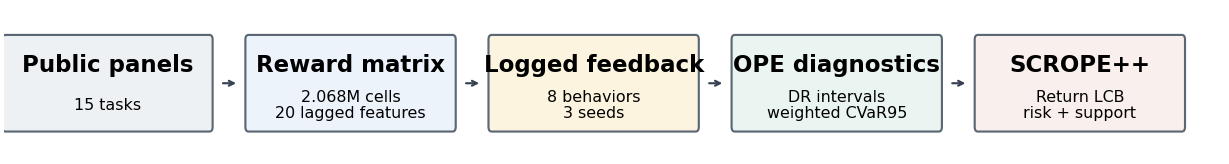
\includegraphics[width=\columnwidth]{pipeline_clean.png}
\caption{FinRisk-OPE pipeline from public panels to selective certification.}
\label{fig:pipeline}
\end{figure}

\section{Related Work}

The central question underlying this work is not how to obtain the highest estimated return from historical data, but what evidence is sufficient to certify a policy before deployment. Existing literature provides important pieces of this answer through support-aware offline learning, off-policy evaluation (OPE), public benchmark design, and financial machine learning. However, these strands are rarely studied within a unified framework for risk-aware policy certification. FinRisk-OPE and SCROPE++ connect them through the common lens of support, reliability, and deployment safety.

\subsection{Support mismatch in offline RL}

Offline reinforcement learning studies policy optimization from fixed datasets without additional interaction. A central challenge is support mismatch: a learned policy may assign probability mass to actions that are weakly represented in the logged data, causing value estimates to depend on unsupported extrapolation. Batch-Constrained deep Q-learning (BCQ) restricts candidate actions toward the observed data distribution \cite{FujimotoMP19}; Bootstrapping Error Accumulation Reduction (BEAR) constrains policy learning through distributional regularization \cite{KumarFSTL19}; Conservative Q-Learning (CQL) learns pessimistic value estimates under distribution shift \cite{KumarZTL20}. Model-based methods such as MOPO and MOReL further incorporate uncertainty-aware pessimism to avoid unreliable regions of learned dynamics \cite{YuTYEZLFM20,KidambiRNNJ20}.

A common conclusion across these approaches is that support deficiency is a first-order deployment risk rather than a secondary implementation detail. Our work adopts this perspective but shifts the objective from policy optimization to policy certification. Rather than asking whether a policy can be learned from historical data, we ask whether available evidence is sufficient to justify deployment. Consequently, support is treated as an explicit evaluation target through effective sample size (ESS), interval coverage, tail-risk reliability, and selective abstention.

\subsection{Off-policy evaluation and risk-aware certification}

Off-policy evaluation estimates the performance of a target policy using data collected by a different behavior policy. Classical approaches include direct modeling (DM), inverse propensity scoring (IPS), self-normalized IPS (SNIPS), clipped importance weighting, and doubly robust (DR) estimation. Recent work has advanced minimax OPE, semiparametric efficiency, adaptive weighting, distributionally robust estimation, and counterfactual learning from logged bandit feedback \cite{SwaminathanJ15,DuanJW20,KallusU20,KallusMWZ22,ZhanHHA21,XieYZ23}. Parallel developments extend OPE from expected reward estimation to risk-sensitive objectives, including quantiles and conditional value-at-risk (CVaR) \cite{ChandakNLBT21,HuangLLA21,TaufiqTCTD22}. Conformal calibration and conformal risk control provide complementary tools for uncertainty quantification and risk guarantees \cite{AngelopoulosBFLS24}.

This literature provides increasingly powerful estimators, yet deployment decisions require more than accurate point estimates. A policy may achieve an attractive estimated return while remaining unsafe because its confidence interval is poorly calibrated, its support is insufficient, or its tail losses are underestimated. Existing methods largely focus on estimation, whereas deployment requires certification. SCROPE++ addresses this gap by combining return evidence, downside-risk evidence, and support evidence into a unified \textsc{Accept}/\textsc{Reject}/\textsc{Abstain} decision framework.

\subsection{Public benchmarks for counterfactual evaluation}

Public benchmarks play a critical role in making offline evaluation reproducible and comparable. D4RL established standardized evaluation protocols for offline RL across simulated control environments \cite{FuKNTL20}. The Open Bandit Dataset and Open Bandit Pipeline introduced logged recommendation datasets with known propensities and reproducible OPE workflows \cite{SaitoAMN21}. More broadly, dataset documentation practices emphasize transparency regarding data sources, collection mechanisms, intended use, and version control \cite{GebruMVWDL21}.

These efforts demonstrate that meaningful evaluation requires a shared and reproducible experimental object. However, finance presents a unique challenge. Public return panels are widely available, but public logged-decision datasets with known propensities and observable counterfactual outcomes are rare. As a result, OPE studies in finance often rely on proprietary data, unverifiable logging assumptions, or evaluation protocols that cannot directly measure counterfactual estimation error.

FinRisk-OPE addresses this reproducibility gap through a semi-synthetic design. Unlike fully simulated environments, rewards correspond to realized market outcomes from public Kenneth French portfolio files rather than model-generated trajectories. At the same time, constructed logging policies provide known propensities, enabling exact OPE evaluation under controlled support conditions. This design intentionally trades behavioral realism for counterfactual observability, allowing reliability questions to be studied under a transparent and reproducible protocol.

\subsection{Financial machine learning and evaluation practice}

Financial machine learning investigates return prediction, factor investing, portfolio construction, shrinkage estimation, and characteristic-based asset pricing \cite{GuKX20,FengGX20,KozakNS20,KellyPS19,FreybergerNW20}. Reinforcement-learning-based financial systems include direct reinforcement trading, deep RL portfolio management, FinRL, FinRL-Meta, and DeepTrader \cite{MoodyS01,DengBKRD17,JiangXL17,LiuYLGW20,LiuYLGW22,WangHTZX21}. These studies motivate many of the contexts and policy classes considered in our benchmark, including momentum strategies, volatility-aware allocation, factor-based selection, and characteristic-driven portfolio rules.

Despite methodological diversity, evaluation remains predominantly backtest-centered. Backtests are useful for measuring historical performance, but they do not directly reveal whether a policy is supported by logged behavior, whether uncertainty estimates are calibrated, or whether downside risk has been underestimated. Consequently, a policy that appears attractive in a retrospective ranking may still be an unsafe deployment candidate.

Our work augments this evaluation paradigm with counterfactual certification. Rather than treating policy assessment as a return-ranking exercise, FinRisk-OPE evaluates whether available evidence is sufficient to support deployment under explicit support and risk constraints.

\subsection{Summary of the Gap}

Existing literature provides the necessary components but not their integration. Offline RL highlights the importance of support. OPE provides estimators for counterfactual value and risk. Public benchmarks establish reproducibility standards. Financial machine learning supplies realistic decision domains and policy classes. What remains missing is a public and reproducible framework that evaluates these components jointly.

FinRisk-OPE fills this gap by combining known logging propensities, exact counterfactual rewards, return-OPE evaluation, coverage diagnostics, tail-risk reliability analysis, and support-aware certification within a single date-frozen protocol. SCROPE++ complements this benchmark by transforming estimation outputs into deployment decisions through selective certification. Together, they shift the focus from estimating performance to certifying whether available evidence is sufficient for safe deployment.

\section{Method}

\subsection{Design overview}

The method has two layers. The first layer is the benchmark construction: convert public portfolio return panels into contextual-bandit tasks with known logging propensities and full-information rewards. The second layer is selective certification: estimate return and downside risk for candidate policies, then certify only policies whose return, risk, and support evidence jointly pass. This separation is important for the paper's applied contribution. The benchmark can be reused with other OPE estimators, while SCROPE++ is one risk-aware certification protocol evaluated on top of it.

\subsection{Problem setup}

We formulate portfolio allocation as a finite-action contextual bandit. At time $t$, the learner observes context $x_t \in \mathbb{R}^d$, chooses action $a_t \in \mathcal{A}$, and receives reward $r_t(a_t)$. A logged sample is
\begin{equation}
    (x_t, a_t, r_t(a_t), \pi_b(a_t|x_t), t),
\end{equation}
where $x_t$ is the lagged market context, $a_t$ is the logged portfolio action, $r_t(a_t)$ is its realized next-period return, $\pi_b(a_t|x_t)$ is the known behavior propensity, and $t$ records chronological order. A deterministic target policy $\pi$ maps contexts to actions. The goal is to estimate expected return
\begin{equation}
    V(\pi)=\mathbb{E}_{t}[r_t(\pi(x_t))]
\end{equation}
and risk functionals such as 95\% conditional value-at-risk loss, denoted CVaR95. The expectation is over evaluation dates, and the CVaR95 loss is lower when downside tail loss is smaller.

\subsection{Benchmark construction}

FinRisk-OPE constructs a reward matrix $R \in \mathbb{R}^{T \times K}$, where $T$ is the number of periods and $K=|\mathcal{A}|$ is the number of portfolio actions. Each entry $R_{t,a}$ is the next-period return of action $a$. We build 15 benchmark tasks: monthly industry allocation, monthly size--book-to-market allocation, monthly size--operating-profitability allocation, monthly size--investment allocation, monthly two-characteristic allocation, daily size-characteristic allocation, daily industry allocation, and daily factor--momentum allocation. All tasks come from Kenneth French Data Library portfolio files.

For each task, the context vector contains only information available before the reward date. The implemented context builder uses 20 lagged summaries of the reward panel, including recent-window means, volatilities, extrema, quantiles, sign rates, and magnitude summaries. The action space is a finite set of portfolio sleeves. Small, medium, and large action spaces are created when a panel contains enough columns, which lets the benchmark test whether certification becomes harder as the decision set grows.

Logged bandit feedback is generated under eight behavior policies: uniform high overlap, softmax high entropy, epsilon-greedy momentum, risk-averse low volatility, return-seeking recent winner, market-state mixed behavior, low-overlap concentration, and adversarial support mismatch. These logging policies are designed to span different overlap conditions. Each log stores the selected action, observed reward, known propensity, support diagnostics, and the full date index. The implemented target-policy library contains one constant policy for each available action, momentum-12, low-volatility-12, mean/volatility-12, and a train-only ridge-return policy.

The benchmark is semi-synthetic in the specific sense needed for OPE evaluation: actions and propensities are generated, but outcomes are empirical market returns. This design gives three properties that real financial logs rarely provide together: known propensities, exact counterfactual rewards within the discrete portfolio action space, and a public data source with source-file hashes.

\subsection{Return and risk OPE}

For a deterministic policy $\pi$, the inverse propensity scoring (IPS) estimator is
\begin{equation}
    \widehat V_{\mathrm{IPS}}(\pi)
    = \frac{1}{n}\sum_{t=1}^{n}
    \frac{\mathbb{I}\{a_t=\pi(x_t)\}}{\pi_b(a_t|x_t)} r_t(a_t),
\end{equation}
Here $n$ is the evaluation sample size, $\mathbb{I}\{\cdot\}$ is the indicator function, $a_t$ is the logged action, $\pi(x_t)$ is the target-policy action, and $\pi_b(a_t|x_t)$ is the behavior propensity. Given reward model $\hat{\mu}(x,a)$ and importance weight $w_t=\mathbb{I}\{a_t=\pi(x_t)\}/\pi_b(a_t|x_t)$, the doubly robust (DR) estimator is
\begin{equation}
    \widehat V_{\mathrm{DR}}(\pi)
    = \frac{1}{n}\sum_{t=1}^{n}
    \left[\hat{\mu}(x_t,\pi(x_t))+
    w_t\{r_t(a_t)-\hat{\mu}(x_t,a_t)\}\right].
\end{equation}
In the DR expression, $\hat{\mu}(x_t,\pi(x_t))$ is the model-predicted reward for the target action, $\hat{\mu}(x_t,a_t)$ is the model-predicted reward for the logged action, and $w_t$ corrects for the difference between the target and behavior policies. The primary released tables use the DR estimator with paired IID and circular block bootstrap intervals. Risk OPE estimates CVaR95 loss from weighted logged returns and computes a one-sided paired-bootstrap upper confidence bound. Because $R$ is fully observed, both return and risk estimates are compared with full-information ground truth.

\subsection{SCROPE++ selective certification}

SCROPE++ converts OPE estimates into certification decisions. It selects among candidate policies only when return, risk, and support evidence jointly pass:
\begin{align}
    \max_{\pi \in \Pi} \quad & \mathrm{LCB}_{0.95}\{\widehat V_{\mathrm{DR}}(\pi)\}\\
    \mathrm{s.t.}\quad
    & \mathrm{UCB}_{0.95}\{\widehat{\mathrm{CVaR}}_{0.95}(\pi)\} \leq \tau, \\
    & \mathrm{ESS}(\pi) \geq \eta, \quad \max_t w_t(\pi) \leq \omega,\\
    & \mathrm{support\ gap}(\pi) \leq \gamma.
\end{align}
Here $\Pi$ is the target-policy class. $\mathrm{LCB}_{0.95}$ and $\mathrm{UCB}_{0.95}$ are 95\% lower and upper confidence bounds, $\tau$ is a baseline-linked CVaR threshold, $\eta$ is a minimum effective-sample-size (ESS) threshold, $\omega$ limits extreme importance weights, and $\gamma$ limits support mismatch. The released configuration uses $\eta=10$, $\omega=50$, and $\gamma=0.995$. The support gap is $1-\min(1,\mathrm{ESS}/n)$, so larger values indicate weaker effective support. SCROPE++ returns ACCEPT if a policy passes the return, risk, and support checks, REJECT if support is adequate but the risk or return check is not met, and ABSTAIN if support is inadequate. This selective design is important in finance: unsupported deployment decisions should not be forced.

Operationally, SCROPE++ proceeds in four steps. First, it evaluates every candidate policy with return and risk OPE on the logged data. Second, it computes support diagnostics from the importance weights induced by the target and behavior policies. Third, it filters policies through support and risk checks before ranking them by return lower confidence bound. Fourth, it reports one of three outputs: ACCEPT if a certifiable policy exists, REJECT if support is adequate but the policy class fails the return or risk check, and ABSTAIN if the evidence is too weak to support certification.

We define a false-safe approval as a decision where a selector accepts or selects a policy, the estimated risk certificate declares the policy safe, $\mathrm{UCB}_{0.95}\{\widehat{\mathrm{CVaR}}_{0.95}(\pi)\}\leq\tau$, but the full-information realized CVaR95 exceeds the same safety threshold. We report false-safe approval among ACCEPT decisions and unsafe acceptance under a common matched-acceptance comparison. These metrics measure the error that matters for deployment: certifying or accepting a policy whose realized tail risk violates the chosen risk threshold.

\subsection{Selective risk certification}

SCROPE++ is evaluated through matched-acceptance comparisons rather than one fixed deployment threshold. The primary comparison fixes the task, behavior, seed, and test-window universe and retains the same number of ACCEPT decisions for every selector. This framing is related to selective prediction, where abstention is evaluated as part of the empirical comparison rather than hidden behind a forced decision for every case \cite{GeifmanE17}.

\subsection{Certification boundary}

SCROPE++ is positioned as an empirical certification protocol. Its risk certificate is interpreted under the calibration of CVaR95 upper bounds on supported policies. FinRisk-OPE therefore reports support, interval coverage, CVaR95 underestimation, false-safe approval, and abstention together, so that certification decisions can be audited against full-information outcomes.

\section{Experiments}

\subsection{Data, tasks, and freeze}

The benchmark is frozen at 2026-04-30 and uses the public Kenneth French ZIP files released with the code package. The released manifest records SHA-256 hashes for all source files. The primary runner produces 50,784 case rows across calibration/test splits and IID/block bootstrap schemes, together with 2,068,330 full-information reward cells. Table~\ref{tab:benchmark_summary} summarizes the 15 public tasks.

\begin{table*}[t]
\centering\scriptsize
\setlength{\tabcolsep}{3pt}
\caption{Current benchmark after filtering and 60-date warmup. Periods and cells cover train, calibration, and test; feature count is 20 for every task.}
\label{tab:benchmark_summary}
\begin{tabular}{lrrrrrrrr}
\toprule
Family & Tasks & Periods & Actions & Features & Train & Cal. & Test & Cells \\
\midrule
Monthly industry & 3 & 694 & 18--48 & 20 & 450 & 108 & 136 & 67,318 \\
Monthly size--B/M & 2 & 654--694 & 26--100 & 20 & 420--450 & 108 & 126--136 & 83,444 \\
Monthly size/profit/invest & 2 & 694 & 26 & 20 & 450 & 108 & 136 & 36,088 \\
Monthly two-characteristic & 3 & 694 & 26 & 20 & 450 & 108 & 136 & 54,132 \\
Daily size characteristic & 3 & 15753 & 26 & 20 & 10640 & 2265 & 2848 & 1,228,734 \\
Daily industry/factor & 2 & 15753 & 7--31 & 20 & 10640 & 2265 & 2848 & 598,614 \\
Total & 15 &  &  &  &  &  &  & 2,068,330 \\
\bottomrule
\end{tabular}
\end{table*}


\subsection{Baselines}

Baselines are chosen to match the deployable information budget. Return-only selection ranks policies by a return lower confidence bound, support-only selection uses support evidence, and risk-only selection ranks policies by the estimated risk bound. All selectors use the same logged contexts, known propensities, candidate policies, test windows, and seeds. The comparison is selector-based because the experiment evaluates certification under fixed logged data.

\subsection{Metrics and statistical protocol}

Metrics follow their deployment role. Coverage measures empirical confidence-interval coverage; effective sample size (ESS) measures logged-policy support; CVaR95 loss is lower when tail loss is smaller; false-safe approval measures risk-certified policies whose realized risk violates the threshold; and unsafe acceptance measures all accepted policies whose realized risk violates the threshold. All confidence intervals and CVaR upper bounds use paired bootstrap resampling on the evaluation window, and all selected-policy outcomes are evaluated against the full-information reward matrix.

\subsection{Implementation details}

The implementation fixes the data freeze, chronological splits, behavior-policy propensities, target-policy library, and selector operating point before comparison. The released package contains the source ZIP files, a SHA-256 manifest, case-level experiment CSVs, generated tables, evidence CSVs, \texttt{export\_paper\_evidence.py}, and \texttt{number\_trace.json}. Bootstrap intervals and CVaR bounds use the same evaluation windows across selectors.

\subsection{Return OPE diagnostics}

Across the return-OPE cases, aggregate results show a familiar tension: estimators with lower point error are not always those with better interval coverage or support behavior. We therefore make support-stratified calibration the main return-OPE table rather than relying on a single estimator leaderboard.

Table~\ref{tab:ope_by_support} reports calibration by ESS bin and bootstrap/calibration method. Standard iid and block intervals substantially under-cover in weak-support bins. Support-stratified conformal calibration restores near-nominal coverage in the lowest ESS bin by widening intervals. The gap between nominal and calibrated coverage indicates that support should be reported alongside point error rather than treated as a nuisance statistic.

\begin{table}[t]
\centering\scriptsize
\setlength{\tabcolsep}{3pt}
\caption{DR interval coverage by ESS. IID, Block, and Cal. are percentages; Cal. applies support-bin offsets to block intervals. Widths are in return units.}
\label{tab:ope_by_support}
\begin{tabular}{lrrrrrr}
\toprule
ESS & $N$ & IID & Block & Cal. & Width & Cal. width \\
\midrule
0--2 & 4798 & 26.28 & 27.45 & 94.60 & 0.1688 & 0.1942 \\
2--5 & 2856 & 68.00 & 68.35 & 96.04 & 0.1081 & 0.1325 \\
5--10 & 1930 & 68.76 & 69.74 & 93.16 & 0.0805 & 0.1233 \\
10--50 & 1049 & 57.77 & 58.91 & 91.42 & 0.0299 & 0.0932 \\
50+ & 2063 & 82.40 & 83.91 & 96.22 & 0.0063 & 0.0096 \\
\bottomrule
\end{tabular}
\end{table}


\begin{figure}[t]
\centering
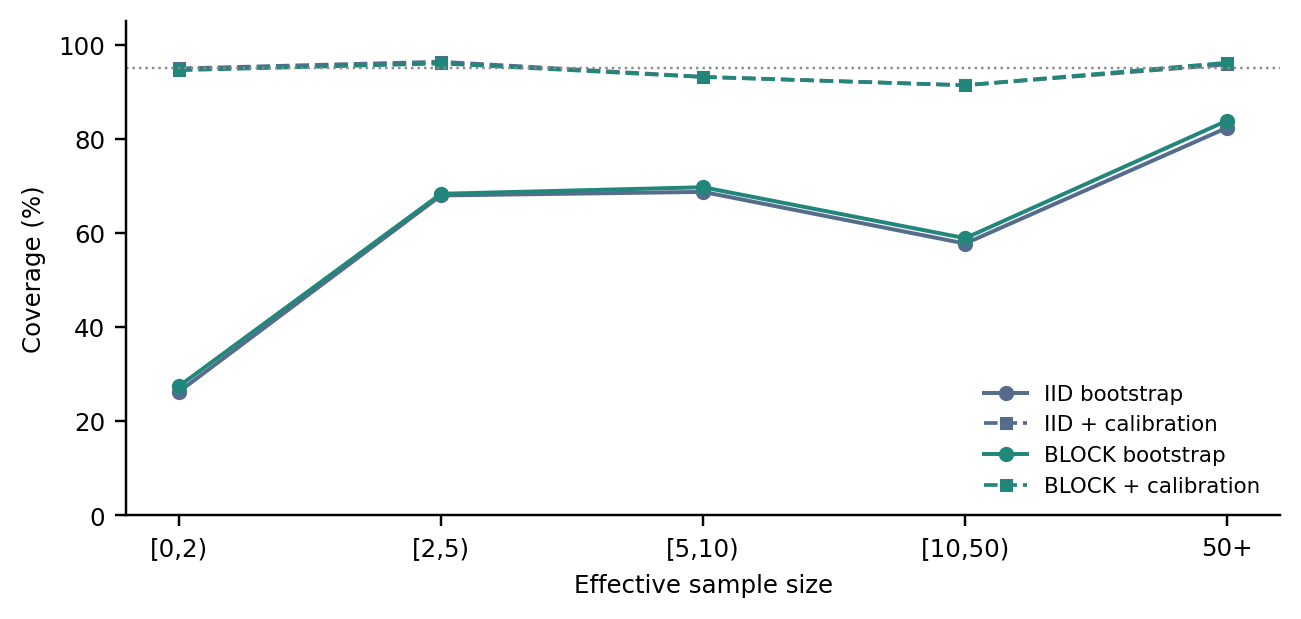
\includegraphics[width=\columnwidth]{coverage_by_ess_clean.png}
\caption{Empirical interval coverage by effective-sample-size (ESS) bin and calibration method.}
\label{fig:coverage_ess}
\end{figure}

\subsection{Risk OPE diagnostics}

CVaR95 estimation error is material across tasks. Test-window underestimation ranges from 66.42\% in the daily industry/factor family to 94.23\% in the monthly size--book-to-market family. Table~\ref{tab:risk_family} summarizes the evidence by task family, while the released evidence CSVs provide case-level diagnostics. These results indicate that downside-risk OPE should be audited alongside return OPE because tail-risk underestimation can change policy-selection conclusions.

\begin{table}[t]
\centering\scriptsize
\setlength{\tabcolsep}{3pt}
\caption{Test-window CVaR95 diagnostics. Underestimation (Under., \%) and MAE exclude undefined risk estimates; median ESS uses all cases.}
\label{tab:risk_family}
\begin{tabular}{lrrrr}
\toprule
Family & Valid & Under. & MAE & ESS \\
\midrule
Monthly industry & 2013 & 86.98 & 0.0849 & 2.34 \\
Monthly size--B/M & 1960 & 94.23 & 0.1051 & 1.00 \\
Monthly size/P/I & 1218 & 89.41 & 0.0752 & 3.97 \\
Monthly two-char. & 1902 & 88.85 & 0.0715 & 4.00 \\
Daily size-char. & 2135 & 74.52 & 0.0123 & 78.58 \\
Daily industry/factor & 1096 & 66.42 & 0.0112 & 56.07 \\
\bottomrule
\end{tabular}
\end{table}


\subsection{SCROPE++ matched-acceptance safety}

\begin{figure}[t]
\centering
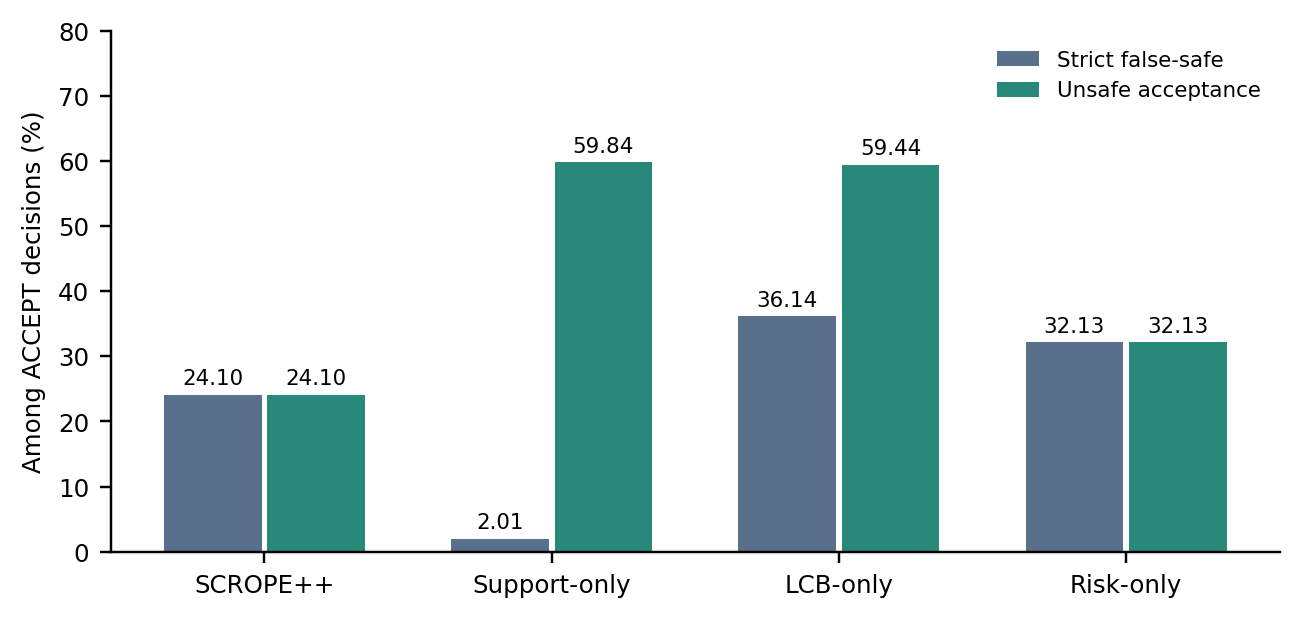
\includegraphics[width=\columnwidth]{matched_acceptance_rates.png}
\caption{Strict false-safe and unsafe-acceptance rates in the matched-acceptance comparison.}
\label{fig:matched_abstention}
\end{figure}

Table~\ref{tab:reviewer_aligned} compares selectors at equal ACCEPT counts. Each selector has 249 ACCEPT decisions out of 360 task--behavior--seed groups. SCROPE++ has an unsafe-acceptance rate of 24.10\%, compared with 59.84\% for support-only, 59.44\% for LCB-only, and 32.13\% for risk-only selection. Strict false-safe rates are reported separately because the selectors do not use identical risk gates. Support-only does not impose the CVaR upper-bound condition when selecting: 149 of its 249 accepted decisions are unsafe, but only 5 also satisfy the estimated-risk condition, yielding 2.01\%. This lower certificate-conditional rate therefore does not indicate safer accepted policies. SCROPE++ enforces the risk gate at acceptance, so its 60 unsafe acceptances are also strict false-safe; unsafe acceptance is consequently the primary cross-selector safety metric.

\begin{table}[t]
\centering\scriptsize
\setlength{\tabcolsep}{3pt}
\caption{Matched-acceptance audit, 360 groups per selector. FS and UA are strict false-safe and unsafe-acceptance percentages among ACCEPT decisions. ABSTAIN includes budget withholding.}
\label{tab:reviewer_aligned}
\begin{tabular}{lrrrrr}
\toprule
Selector & Accept & Reject & Abstain & FS & UA \\
\midrule
SCROPE++ & 249 & 62 & 49 & 24.10 & 24.10 \\
Support only & 249 & 0 & 111 & 2.01 & 59.84 \\
LCB only & 249 & 0 & 111 & 36.14 & 59.44 \\
Risk only & 249 & 0 & 111 & 32.13 & 32.13 \\
\bottomrule
\end{tabular}
\end{table}

Because SCROPE++ reports rejection and abstention explicitly, its safety rates should be interpreted together with acceptance and refusal behavior rather than as unconditional trading dominance.

\subsection{Reproducibility material}

The public source data are available from the Kenneth R. French Data Library at \url{https://mba.tuck.dartmouth.edu/pages/faculty/ken.french/data_library.html}. The FinRisk-OPE code, frozen inputs, reference outputs, generated tables, and number-tracing artifacts are available at \url{https://github.com/666lyc-123/FinRisk-OPE}. The repository records source and code hashes, pins the software environment, and provides an automated full-pipeline verification workflow.

\section{Conclusion}

This paper reframes financial offline policy selection as a policy-certification problem rather than a return-ranking problem. While financial decision systems are often evaluated through retrospective backtests, deployment requires stronger evidence: a policy must be supported by the logged data, its uncertainty estimates must remain reliable under distribution shift, and its downside risk must be acceptably bounded. FinRisk-OPE was developed to make these requirements measurable and reproducible.
The empirical results reveal a consistent pattern across financial tasks. Accurate return estimation alone is insufficient for reliable deployment. Policies operating in weak-support regions frequently exhibit degraded interval coverage, while downside-risk measures such as CVaR95 can be substantially underestimated even when expected-return estimates appear accurate. These findings suggest that support deficiency and tail-risk misestimation are not isolated technical issues but fundamental obstacles to trustworthy financial off-policy evaluation.
To address this challenge, we introduced SCROPE++, a selective certification framework that combines support evidence, return uncertainty, and downside-risk assessment into a unified deployment decision. Rather than forcing a binary recommendation, SCROPE++ explicitly allows abstention when the available evidence is insufficient. In financial settings, such abstention should be viewed as a safety mechanism rather than a failure mode, reflecting the principle that uncertainty itself is actionable information.
Financial offline learning should therefore be evaluated by whether counterfactual evidence justifies deployment, rather than by return rankings alone. By combining known propensities, exact counterfactual rewards, support diagnostics, risk estimation, and selective certification within a date-frozen public benchmark, FinRisk-OPE provides a reproducible setting for this question.

Several limitations remain. Logging policies are constructed rather than recovered from investor behavior, and rewards omit transaction costs and market impact. The benchmark does not yet cover transaction-level, order-book, or product-interaction environments. Future work should add validated real-world logs, execution frictions, and richer distributional-risk estimators. The central implication is that profitable backtests still require support, uncertainty, and downside-risk certification before deployment.

{\scriptsize
\bibliographystyle{IEEEtran}
\bibliography{finrisk_ope_refs}
}

\end{document}
